\documentclass[../../../../main.tex]{subfiles}
\begin{document}

\begin{flushright}
\footnotesize\textit{【自動文字起こし・要確認】}
\end{flushright}

\noindent
[\textbf{解}] $X = \frac{x}{a}, Y = \frac{y}{b}$ なる変換をほどこす.

$P$ は $P'(\cos u, b \sin u)$ に, 楕円は $X^2 + Y^2 = 1$ にうつり, $OP$ のはいった部分は下図斜線部(この面積 $S'$ とする)にうつる. 変換の定義から
\[
S = S' ab \quad \cdots \text{①}
\]
であり,
\[
S' = \frac{1}{2} u
\]
だから①に代入して
\[
S = \frac{1}{2} ab u
\]
$\frac{dS}{dt} = 1$ より
\[
\frac{dS}{dt} = \frac{1}{2} ab \frac{du}{dt} = 1
\]
\[
\therefore \frac{du}{dt} = \frac{1}{ab}
\]
\[
du = \frac{1}{ab} dt
\]
積分して
\[
u = \frac{1}{ab} t + C \quad (C \text{:定数})
\]
$t=0$ で $u=0$ より $C=0$ だから, \underline{$u = \frac{1}{ab} t$} である.

\begin{center}
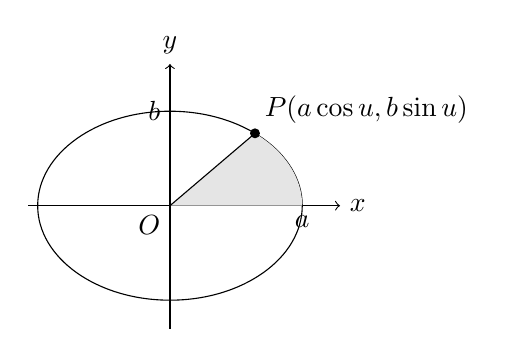
\begin{tikzpicture}[scale=1.2]
    \draw[->] (-1.5,0) -- (1.8,0) node[right] {$x$};
    \draw[->] (0,-1.3) -- (0,1.5) node[above] {$y$};
    \node[below left] at (0,0) {$O$};
    \draw (0,0) ellipse (1.4cm and 1.0cm);
    \fill[gray!20] (0,0) -- (1.4,0) arc (0:50:1.4cm and 1.0cm) -- cycle;
    \draw (0,0) -- (50:1.4cm and 1.0cm) node[above right] {$P(a\cos u, b\sin u)$};
    \fill (50:1.4cm and 1.0cm) circle (1.5pt);
    \node[below] at (1.4,0) {$a$};
    \node[left] at (0,1.0) {$b$};
\end{tikzpicture}
\hspace{1cm}
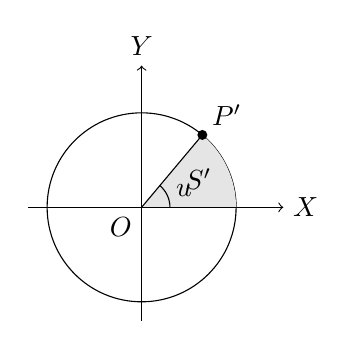
\begin{tikzpicture}[scale=1.2]
    \draw[->] (-1.2,0) -- (1.5,0) node[right] {$X$};
    \draw[->] (0,-1.2) -- (0,1.5) node[above] {$Y$};
    \node[below left] at (0,0) {$O$};
    \draw (0,0) circle (1.0cm);
    \fill[gray!20] (0,0) -- (1.0,0) arc (0:50:1.0cm) -- cycle;
    \draw (0,0) -- (1.0,0);
    \draw (0,0) -- (50:1.0cm) node[above right] {$P'$};
    \fill (50:1.0cm) circle (1.5pt);
    \draw (0.3,0) arc (0:50:0.3cm);
    \node at (0.45,0.18) {$u$};
    \node at (0.6,0.3) {$S'$};
\end{tikzpicture}
\end{center}

\newpage

\end{document}
